\subsection{Normalization to HESE Flux}
\label{sec:norm2HESE}
% \begin{itemize}
%  \item my way: average Lpeak, average t90, integrate over ???
%  \item same result.
%  \item table of results??? once I have final dataset?
%  \item plot
%  \item influence of emin: upsilon but also not considering events with
% E<E(1+z)???
% \end{itemize}
The luminosity is drawn according to the luminosity function fitted to
gamma-ray data, assuming the neutrino luminosity function to follow the
same shape. However, a normalization factor might be needed to trim it to the
correct energies and consequently to the correct number of neutrinos to produce
the HESE flux. ($N_\text{exp}^\nu \propto \hat{E}_{\nu, \text{total}} \propto
L_\text{Peak}$). Equation \ref{eq:Nexp_wZB} evolves to
% \begin{equation}
% \label{eq:Nexp_wZB_wEps}
%  N_\text{exp}^\nu = \sum_i\frac{dF_P(E_i)}{dE_i} \cdot
% \frac{OneWeight_i}{N_\text{generated}}
% \end{equation}
\begin{eqnarray}
\label{eqn:Nexp_wZB_wEps}
 N_\text{exp}^\nu &= & \epsilon \cdot \sum_i \cdot \frac{\hat{E}_{\nu,
\text{total}}}{4 \pi
d_l^2\Upsilon\left(\hat{E}_{min}, \hat{E}_\text{cut}\right)} \cdot
E_i^{-\gamma}
\text{exp} \left( - \frac{E_i \cdot (1+z)}{\hat{E}_\text{cut}} \right) \cdot
(1+z)^{3 - \gamma}
\frac{OneWeight_i}{N_\text{generated} \cdot \frac{A_{ZB}}{4 \pi}} \\
&= & \epsilon^* \cdot \sum_i \cdot \frac{\hat{E}_{\nu, \text{total}}}{4 \pi
d_l^2} \cdot
E_i^{-\gamma}
\text{exp} \left( - \frac{E_i \cdot (1+z)}{\hat{E}_\text{cut}} \right) \cdot
(1+z)^{3 - \gamma}
\frac{OneWeight_i}{N_\text{generated} \cdot \frac{A_{ZB}}{4 \pi}}
\label{eqn:Nexp_wZB_wEpsStar}
\end{eqnarray}
Once $\hat{E}_{min}$ (chapter ???) and $\hat{E}_\text{cut}$ are determined,
$\Upsilon$ is a constant for every GRB which can be included in an effective
normalization factor
\begin{equation}
\epsilon^* =
\frac{\epsilon}{\Upsilon\left(\hat{E}_{min}, \, \hat{E}_\text{cut}\right)}
\end{equation}
Due to the effective normalization factor it is redundant to calculate the
constant $\Upsilon$. However, a different $\epsilon^*$ needs to be determined
for different $\hat{E}_{min}$. The impact of choosing different minimal
energies is studied in chapter ???.

There are two ways to determine $\epsilon$ - a Monte Carlo based and a semi
analytic one.
\subsubsection{$\epsilon^*$ - Monte Carlo Based}
This approach was followed by Nora Strotjohann. Given the different
spectra fitted to the HESE flux (chapter \ref{sec:GRBSpectra}), a different
number of neutrinos per year are expected due to GRBs. Using the nugen
simulation without the GRB simulation one can simply calculate the number of
neutrinos using the spectra fitted at earth. They are displayed in figure
\ref{fig:Espectra}. Their shape is quite similar at high energies at which the
HESE events were found. However, the curves diverge quite significantly at
lower energies leading to different predictions about the number of neutrinos
one could expect from GRBs on OFU level.

\begin{figure}[h]
\centering
 \captionsetup{width=.68\textwidth}
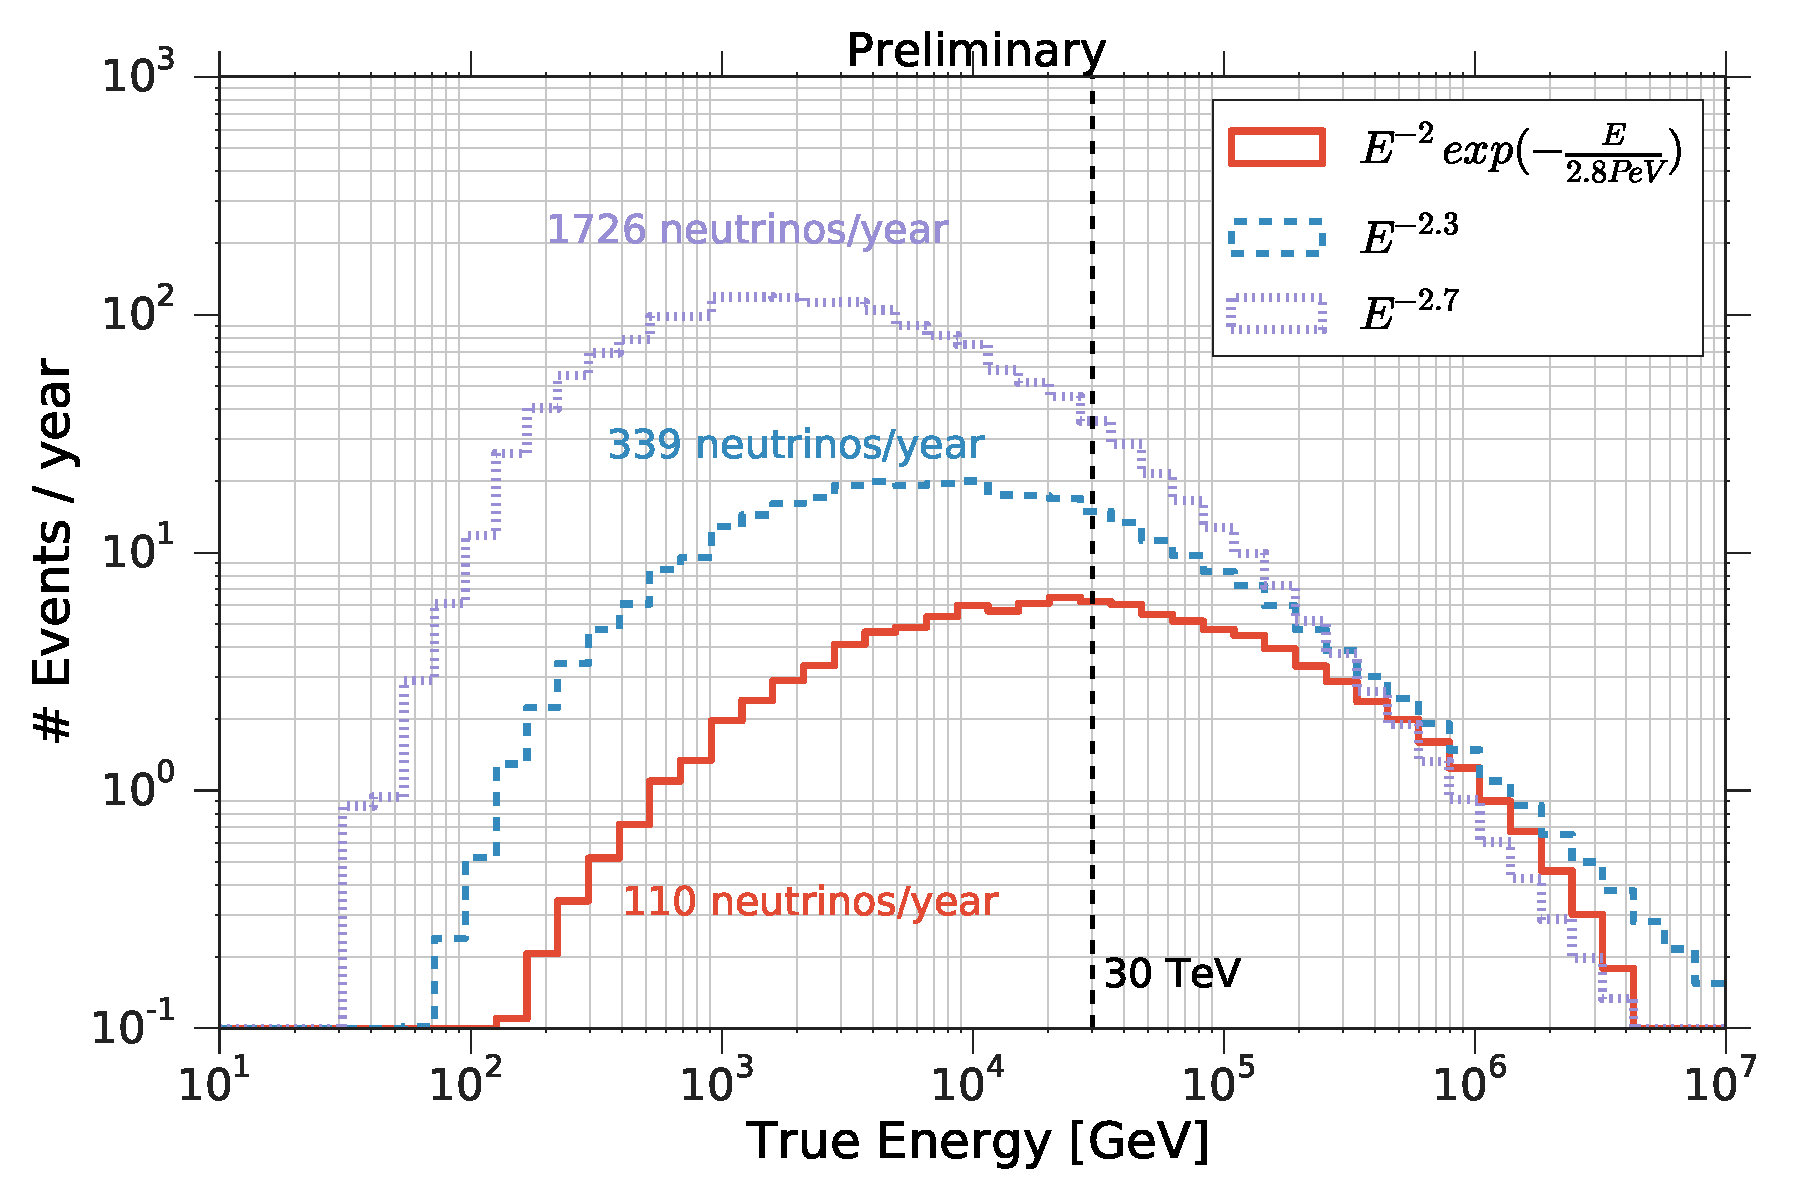
\includegraphics[width=0.68\textwidth]{fig/Spectra_on_OFU.pdf}
    \caption{The three different spectra fitted to the HESE events on OFU
level. The true neutrino energy is used. The number of expected neutrinos is
highly dependent on the chosen spectrum.}
\label{fig:Espectra}
\end{figure}

To determine $\epsilon^*$ up to 5 million GRBs ($N_\text{GRB, sim}$) are
simulated with $\epsilon^*$ set to one. The sum over $N_\text{exp}^\nu$ of all
GRBs is renormalized to the number of expected GRBs per year
$N_\text{GRB, yr}$ and needs to reproduce the number of expected neutrinos on
OFU level.
\begin{equation}
\epsilon^*  = \frac{N_\text{exp}^\nu (\epsilon^* = 1) \cdot
\frac{N_\text{GRB, yr}}{N_\text{GRB, sim}}}{N_{\text{exp, OFU}}^\nu}
\end{equation}
The final result depends on the number of expected GRBs per year which is an
uncertain number. Fortunately, it is a linear factor and $\epsilon^*$ can be
changed easily with the knowledge with which $N_\text{GRB, yr}$ it was
calculated.
\begin{equation}
 \epsilon_\text{new}^* = \epsilon^* \cdot \frac{N_\text{GRB,
yr}^\text{new}}{N_\text{GRB,yr}}
\end{equation}



\subsubsection{$\epsilon^*$ - Semi-Analytic Approach}
The second approach integrates over the expected differential fluxes in energy
from all GRBs up to the maximal chosen redshift ($z_{max}=8$) under
consideration of their redshift distribution.
\begin{eqnarray}
 \Phi_\text{GRB} &=& \int_{z=0}^{z=8} dz \, R(z) \cdot \frac{dF_P \left(z,  E,
\hat{E}_{\nu, \text{total}} \left(\hat{t}_{90}, \, L_\text{Peak}\right)
\right)}{dE} \\
&=& \int_{z=0}^{z=8} dz \, R(z) \cdot \frac{\hat{E}_{\nu, \text{total}}}{4 \pi
d_l^2(z)} \cdot
E_i^{-\gamma}
\text{exp} \left( - \frac{E_i \cdot (1+z)}{\hat{E}_\text{cut}} \right) \cdot
(1+z)^{3 - \gamma}
\end{eqnarray}
The final result needs to equal the measured fluxes on earth over the  whole
energy range and the flux is recalculated for 100 energy values between $10$
and $10^9$ GeV evenly spaced in $\text{log} E$.

Next to the redshift of the GRBs and the energy of the neutrinos the signal
expectation is dependent on the
total energy in neutrinos and thus the peak luminosity and the $\hat{t}_{90}$
values. The average value is calculated based on an average time window and
peak luminosity. The average time window $<\hat{t}_{90}>$ was determined out of
5 million drawn values while the average peak luminosity is calculated
according to
\begin{equation}
\begin{align}
 <L_\text{Peak}> &=
\frac{\int_{L_\text{Peak}^{min}}^{L_\text{Peak}^{max}} L_\text{Peak}
\cdot \Phi(L_\text{Peak})
d\text{log}_{10}L_\text{Peak}}{\int_{L_\text{Peak}^{min}}^{L_\text{Peak}^{max}
}\Phi(L_\text{ Peak})
d\text{log}_{10}L_\text{Peak}}\\
&= \frac{\int_{L_\text{Peak}^{min}}^{L_\text{Peak}^{max}} L_\text{Peak}
\cdot
\frac{\Phi(L_\text{Peak})}{L_\text{Peak} \text{ ln}(10)}
dL_\text{Peak}}{\int_{L_\text{Peak}^{min}}^{L_\text{Peak}^{max}}\frac{
\Phi(L_\text{ Peak})}{L_\text{Peak}
\text{ ln}(10)} dL_\text{Peak}}\\
&=
\frac{\int_{L_\text{Peak}^{min}}^{L_\text{Peak}^{max}}\frac{\Phi(L_\text{
Peak})}{\text{ln} (10)}
dL_\text{Peak}}{\int_{L_\text{Peak}^{min}}^{L_\text{Peak}^{max}}\frac{
\Phi(L_\text{ Peak})}{L_\text{Peak}
\text{ ln}(10)} dL_\text{Peak}}
\end{align}
\end{equation}

%table with average values ???


The co-moving rate density $R(z)$ includes a normalization to the number of
expected GRBs according to said model. If a different number of GRBs is
assumed, then the resulting flux needs to be adjusted by an according factor.

This flux of all GRBs up to a redshift of eight needs to reproduce the HESE
flux over the whole energy range (Fig. \ref{fig:Phi_norm}). This can be
achieved for the two spectra without a cut-off.
However, the HESE flux can not be reproduced at very high energies using the
same
exponential cut-off for all GRBs at all redshifts. $\hat{E}_\text{cut}$ was
chosen such that an exact agreement was reached for the most part of the energy
range accepting a disagreement in the tail. Possibly, one could determine an
energy dependent $\epsilon^*$. However, given the few numbers of events at
these energies and the lack of knowledge of the exact shape of the cut-off due
to missing HESE statistic this extra complication was not attempted.
\begin{equation}
 \epsilon^* = \frac{\Phi_\text{HESE}(E)}{\Phi_\text{GRB}(E)}
\end{equation}
The effective efficiency factor can be applied in the further simulation to
each GRB using equation \ref{eqn:Nexp_wZB_wEpsStar}.

Both methods of determining $\epsilon^*$ agree in the order of 1\%. The 
disagreement could result from a random extra bright GRB in the sample used in 
the Monte Carlo based method and / or the calculation precision set for the 
semi-analytic approach.
\begin{figure}[h]
 \centering
 \captionsetup{width=.9\textwidth}
\subfloat[$\hat{E}_{min}$ was set to 1.\label{fig:Phi_norm}]{%
 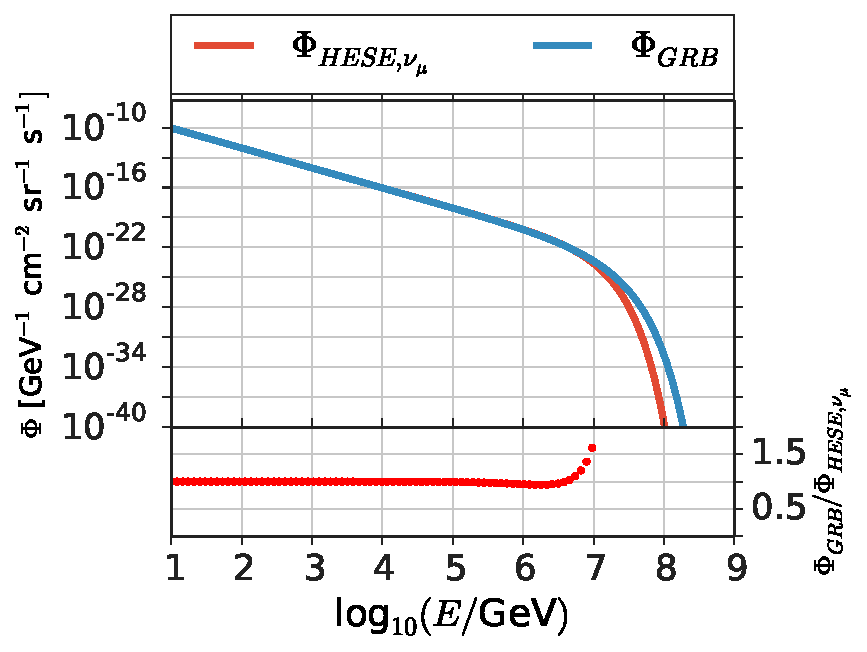
\includegraphics[width=0.45\textwidth]{fig/Phi_norm_gamm2.pdf}}
\subfloat[$\hat{E}_{min}$ was set to $10$ 
TeV.\label{fig:Phi_norm_Emin}]{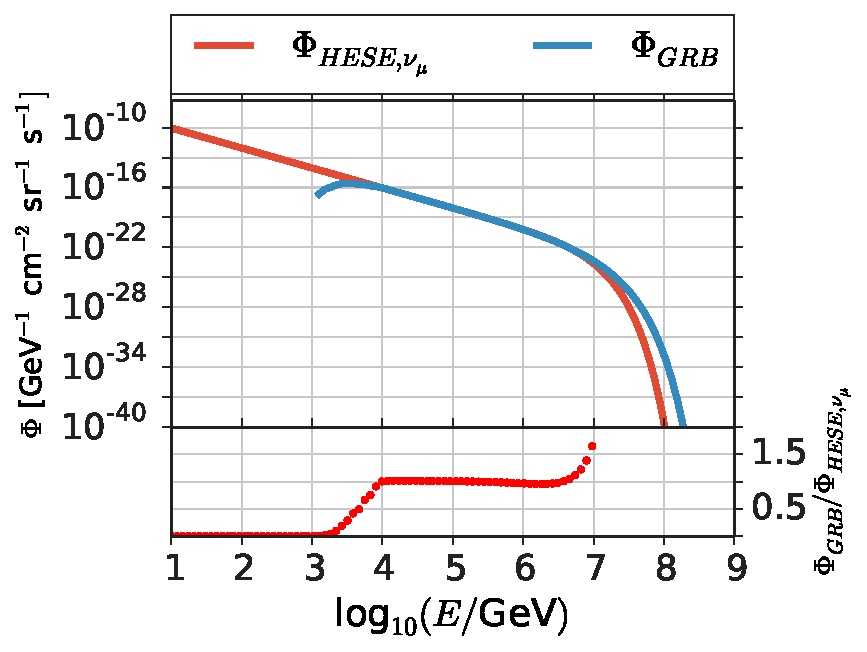
\includegraphics[width=0.45\textwidth]{%
fig/Phi_norm_gamm2_Emin.pdf}}
 \caption{Upper plot: The differential flux in energy for the HESE spectrum
($E^{-2}$ with cut-off) and the spectrum produced by all GRBs up to a redshift
of 8. \\
Lower plot: ratio between the GRB flux and the HESE flux. The ratio should be
queal to one.}
\end{figure}
% emin plot with Emin=10000???



\subsubsection{Influence of $\hat{E}_{min}$}
The influence of the minimal neutrino energy from a GRB has two effects.

The constant $\Upsilon$ in eq. \ref{eqn:Nexp_wZB_wEps} becomes smaller the more
stringent the energy cut is (Eq. \ref{eq:Etotal}) leading to a smaller
efficiency factor $\epsilon$ as the flux at each energy needs to
reproduce the HESE flux. The effective efficiency factor $\epsilon^*$ will stay
the same.
Using the example of $\hat{E}_{min} = 10 \text{ TeV}$ shown in figure
\ref{fig:Phi_norm_Emin}, $\epsilon^*$ was chosen such that an agreement was
found for as large an energy range as possible. Considering all energies (Fig.
\ref{fig:Phi_norm}) $\epsilon^*=0.149$ was determined while applying a minimal
energy leads to  $\epsilon^*=0.151$. The discrepancy of about 1.5 \%  is
probably due to the precision of agreement between the two fluxes required in
the procedure. \textbf{can i do better? I think that I did. checkout 
$emin_redon.ipynb$}

The other effect can be seen at low energies at which the GRB flux drops to
zero. No events with energies
\begin{equation}
 E_\nu \leq \frac{\hat{E}_{min}}{1+z}
\end{equation}
can exist in the detector if a minimal neutrino energy cut at source is
applied. The GRB flux transitions from an agreement with the HESE flux towards
no flux at all because the cut effects are redshift dependent. Neutrinos 
with higher
energies are more effected the  closer to earth a GRB is assumed to be.

In summary, the effect of a different $\hat{E}_{min}$ on the final flux per
energy is non existent. However, events will be lost at lower energies. 

%result table ???

